\documentclass[12pt,a4paper]{report}
\usepackage[utf8]{inputenc}
\usepackage[spanish]{babel}
\usepackage{amsmath}
\usepackage{amsfonts}
\usepackage{amssymb}
\usepackage{lmodern}
\usepackage{amsmath}
\usepackage{enumerate}
\usepackage[left=2cm,right=2cm,top=2cm,bottom=2cm]{geometry}
\usepackage{graphicx}
\usepackage{algpseudocode}
\usepackage{stackrel}
\renewcommand{\theequation}{\arabic{equation}}
\newcounter{neq}
\providecommand{\abs}[1]{\lvert#1\rvert}
\newcommand{\QED}{\hfill \textit{\textbf{Q.E.D.}}}
\author{Agustin Curto, agucurto95@gmail.com}
\title{Resumen de teórico \\ Base de Datos}
\date{2016}

\begin{document}
\maketitle
\tableofcontents

\chapter{Modelado Entidad - Relación}
	\section{Conjuto de Entidades}
		\begin{itemize}
			\item Una \textbf{entidad} es un objeto que existe y es distinguible de los otros objetos. Las entidades tienen atributos.
			\par \underline{Ejemplo:} una persona tiene nombres y direcciones.
			\item Un \textbf{conjunto de entidades} es un conjunto de entidades del mismo tipo (i.e. Con los mismos atributos) que comparte las mismas propiedades.
			\par \underline{Ejemplo:} conjunto de todas las personas con los atributos del ejemplo anterior.
			\item Un \textbf{dominio} es el conjunto de valores permitidos para cada atributo. 
			
			\item Tipos de atributos:
				\begin{itemize}
					\item Atributos Simples y compuestos.
					\item Atributos uni-valorados y multi-valorados
					\item Atributos derivados, pueden computarse de otros atributos.
				\end{itemize}
		\end{itemize}
		
		\subsubsection{Notaciones de diagrama}
			\begin{figure}[htb]
				\centering
				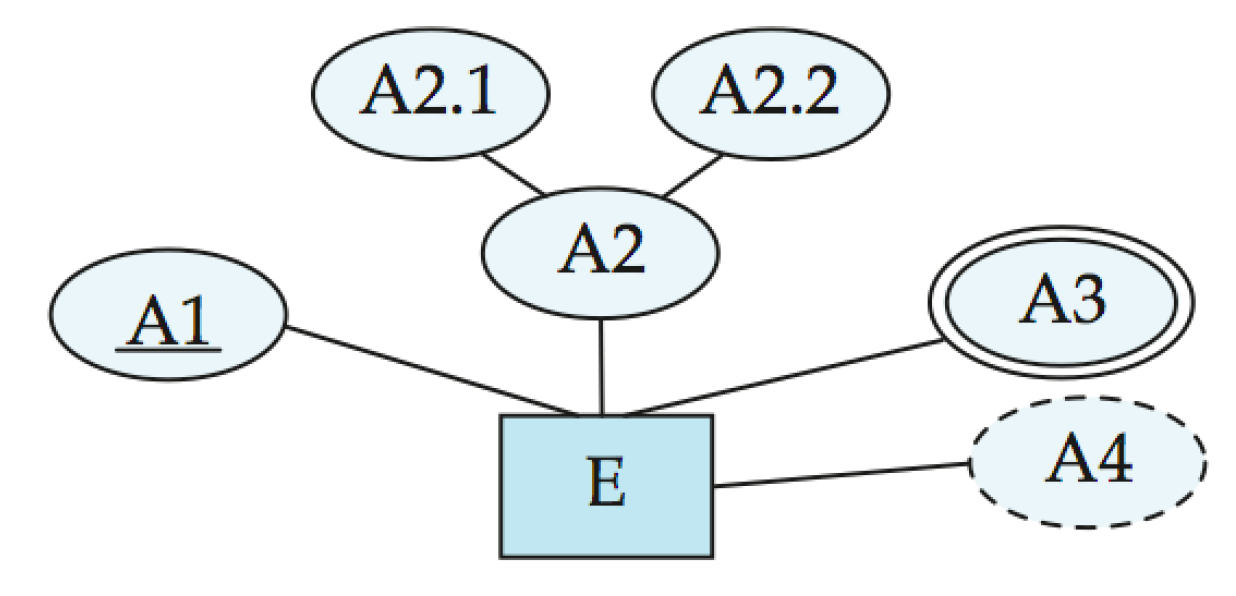
\includegraphics[width=6cm, height=4cm]{./imagenes/entidad.png}
				\caption{Entidad de nombre E, Atributo simple A1, Atributo compuesto A2, Atributo multivalorado A3, Atributo derivado A4, Clave primaria A1}
			\end{figure}

	\section{Claves}
		\begin{itemize}
			\item Una \textbf{superclave} de un CE es un conjunto de uno o más atributos cuyos valores unívocamente determinan cada entidad.
			\item Una \textbf{clave candidata} de un CE es una superclave minimal (i.e. si se quita atributo dejamos de tener superclave).
			\item Una \textbf{clave primaria} es aquella seleccionada de entre todas las claves candidatas que puedan existir.
		\end{itemize}
		
	\section{Correspondencia de cardinales}
		\begin{itemize}
			\item \textbf{Conjuntos de relaciones uno-uno:} una entidad de \textbf{E1} está asociada con a lo más una entidad de \textbf{E2} vía una relación \textbf{R}. Una entidad de \textbf{E2} está asociada con a lo más una entidad de \textbf{E1} vía \textbf{R}.
			\item \textbf{Conjuntos de relaciones uno-varios / varios-uno:} una entidad de \textbf{E1} está asociada con ninguna o varias entidades de \textbf{E2} vía una relación \textbf{R}. Una entidad de \textbf{E2} está asociada con a lo más una entidad de \textbf{E1} vía \textbf{R}.
			\item \textbf{Conjuntos de relaciones varios-varios:} una entidad de \textbf{E1} está asociada con ninguna o varias entidades de \textbf{E2} vía \textbf{R}. Una entidad de \textbf{E2} está asociada con a lo más una entidad de \textbf{E1} vía \textbf{R}.
		\end{itemize}
		
		\begin{center}
			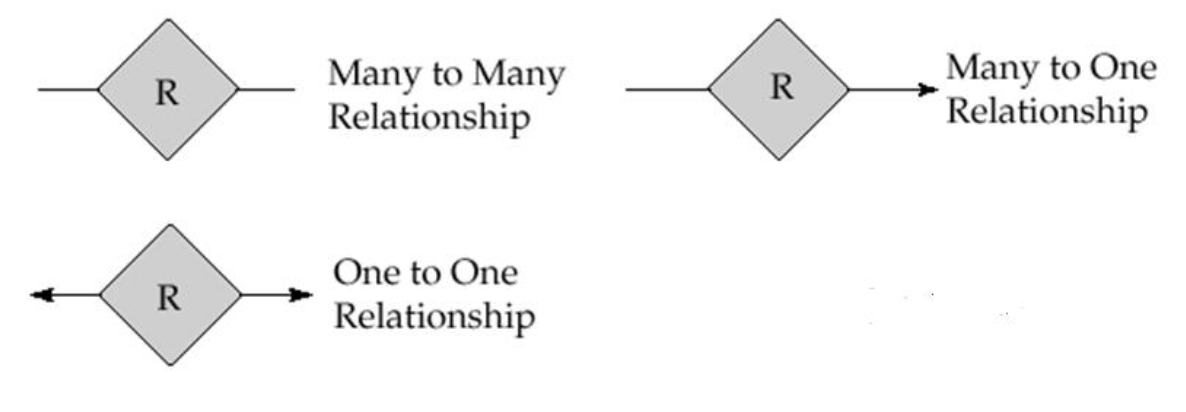
\includegraphics[width=10cm, height=4cm]{./imagenes/correspondencia.png}
		\end{center}
		
	\section{Formas de participación}
		\begin{itemize}
			\item \textbf{Participación total:} toda entidad en el conjunto de entidades participa en al menos una relación en el conjunto de relaciones. Es indicada por una línea doble.
			\par \underline{Ejemplo:} participación de caja de ahorro en cliente es total. Toda caja de ahorro debe tener clientes asociados.
			\item \textbf{Participación parcial:} algunas entidades no participan en alguna relación en el conjunto de relaciones.
			\par \underline{Ejemplo:} participación de instructor en supervisor es parcial.
		\end{itemize}
		
	\section{Conjunto de entidades débiles}
		Un CE que no tiene una clave primaria en el conjunto de sus atributos, se llama \textbf{conjunto de entidades débiles}. La existencia de un CE débiles depende de la existencia de un CE fuertes llamado \textbf{CE identificador}. 
		\vspace{5mm}
		\par \underline{Ejemplo:} ¿En el caso de libro-biblioteca cuál sería el CE identificador?
		\vspace{2.5mm}
		\par Hay un CR varios-uno entre CE débil y CE identificador, donde el CE débil tiene participación total, a este CR se le llama \textbf{CR de identificación}. El mismo se representa con un diamante doble.
		\par El \textbf{discriminador} de un CE débiles es un conjunto de atributos que permite distinguir entre todas las entidades de un CE débiles asociadas a la misma entidad fuerte. 
		\par Para identificar las entidades débiles se forma la clave primaria del CE con la clave primaria del CE identificador más el discriminador del CE débiles.
		
	
		
\end{document}